% Prepublication manuscript source. Local-only working copy.
% Public-facing terminology deliberately excludes internal program codenames.
\documentclass[10pt,a4paper]{article}

\usepackage[a4paper,top=21mm,bottom=23mm,left=22mm,right=22mm]{geometry}
\usepackage[T1]{fontenc}
\usepackage{lmodern}
\usepackage{microtype}
\usepackage{amsmath,amssymb,mathtools}
\usepackage{graphicx}
\usepackage{booktabs}
\usepackage{tabularx}
\usepackage{array}
\usepackage{multirow}
\usepackage{float}
\usepackage{enumitem}
\usepackage[table]{xcolor}
\usepackage{tikz}
\usetikzlibrary{arrows.meta,positioning,calc,fit,backgrounds}
\usepackage{caption}
\usepackage{titlesec}
\usepackage{fancyhdr}
\usepackage{seqsplit}
\usepackage{xurl}
\usepackage{hyperref}

\definecolor{Ink}{HTML}{17202A}
\definecolor{Slate}{HTML}{4D5B66}
\definecolor{Rule}{HTML}{B7C0C7}
\definecolor{PassBlue}{HTML}{356A8A}
\definecolor{PassPale}{HTML}{DFEBF2}
\definecolor{FailPale}{HTML}{F0F1F2}
\definecolor{UnopenedPale}{HTML}{FAF7EE}
\definecolor{Warn}{HTML}{A36A1F}
\definecolor{LinkBlue}{HTML}{245A7A}

\hypersetup{
  colorlinks=true,
  linkcolor=LinkBlue,
  citecolor=LinkBlue,
  urlcolor=LinkBlue,
  pdftitle={Sensitivity Without Reproducibility: A Measurement Boundary for an Operator-Valued Representation Instrument in Qwen Models},
  pdfauthor={Aoi Kawasaki},
  pdfsubject={Cross-presentation measurement boundary for an operator-valued representation instrument in Qwen models},
  pdfkeywords={mechanistic interpretability, representation measurement, visible-state intervention, naturality square, split-half reproducibility, Qwen}
}

\setlength{\parindent}{1.2em}
\setlength{\parskip}{0pt}
\setlength{\tabcolsep}{4.5pt}
\renewcommand{\arraystretch}{1.10}
\setlength{\textfloatsep}{10pt plus 2pt minus 2pt}
\setlength{\intextsep}{10pt plus 2pt minus 2pt}
\setlength{\floatsep}{8pt plus 2pt minus 2pt}
\captionsetup{skip=4pt}
\titlespacing*{\section}{0pt}{2.5ex plus .6ex minus .2ex}{1.0ex}
\titlespacing*{\subsection}{0pt}{1.8ex plus .4ex minus .2ex}{.7ex}
\titlespacing*{\paragraph}{0pt}{1.1ex plus .2ex minus .1ex}{.7em}
\setlist[itemize]{leftmargin=5.2mm,itemsep=1.5pt,topsep=3pt}
\setlist[enumerate]{leftmargin=6.4mm,itemsep=1.5pt,topsep=3pt}
\newcolumntype{Y}{>{\raggedright\arraybackslash}X}
\newcolumntype{C}[1]{>{\centering\arraybackslash}p{#1}}

\pagestyle{fancy}
\fancyhf{}
\fancyhead[L]{\footnotesize\itshape Sensitivity Without Reproducibility}
\fancyhead[R]{\footnotesize Aoi Kawasaki}
\fancyfoot[C]{\footnotesize \thepage}
\renewcommand{\headrulewidth}{0.3pt}
\renewcommand{\footrulewidth}{0pt}
\setlength{\headheight}{13pt}
\fancypagestyle{plain}{%
  \fancyhf{}%
  \fancyfoot[C]{\footnotesize \thepage}%
  \renewcommand{\headrulewidth}{0pt}%
}

\newcommand{\PASS}{\textsc{pass}}
\newcommand{\FAIL}{\textsc{fail}}
\newcommand{\UNOPENED}{\textsc{unopened}}
\newcommand{\NOTQUAL}{\textsc{not qualified}}
\newcommand{\code}[1]{\texttt{\detokenize{#1}}}
\newcommand{\hash}[1]{\texttt{\seqsplit{#1}}}
\newcommand{\PassCell}{\cellcolor{PassPale}\textcolor{PassBlue}{\ensuremath{\checkmark}}}
\newcommand{\FailCell}{\cellcolor{FailPale}\textcolor{Slate}{\ensuremath{\times}}}

\title{\textbf{Sensitivity Without Reproducibility}\\[5pt]
\large A Measurement Boundary for an Operator-Valued\\
Representation Instrument in Qwen Models}
\author{Aoi Kawasaki\\[2pt]
\small Independent Researcher\\[-1pt]
\small \href{https://github.com/Udonburo}{github.com/Udonburo}}
\date{31 August 2026\\[2pt]
\small Technical Report, Version 1.0\\[-1pt]
\small Not peer reviewed.}

\begin{document}
\maketitle

\begin{abstract}
Cross-instance mechanistic claims built from internal representation observables require measurements that are not only sensitive to controlled perturbations but also re-estimable across independent presentation changes. We use \emph{reproducibility} in this protocol-defined cross-presentation sense, not to denote independent-laboratory replication. We studied a phase-indexed binary register in a frozen Qwen checkpoint panel, separating explicit transition following, demonstration-conditioned register behavior, visible-state intervention use, operator-valued representation measurement, and representation--function coupling. Qwen3.5-27B and Qwen3.6-27B passed the behavioral ladder through visible overwrite propagation, whereas Qwen3-14B and Qwen3.8-27B failed an upstream transition gate and were not tested downstream. On Qwen3.6-27B, a rank-4 local-frame paired ridge path-operator packet qualified on an initial bounded substrate using independently generated, disjoint nuisance halves and a matched broken-square control. We then froze a 20-block requalification across rollout depths 2, 4, 6, and 8. Broken-square sensitivity was retained in 59 of 60 layer-blocks, but only 5 of 20 blocks satisfied the prospectively frozen all-three-layer map qualification, with split-half path-map spectral re-estimation as the limiting gate. The behavioral stage therefore remained unopened, and no representation--function association was estimated. The result does not establish the absence of hidden state, internal naturality, or useful representation geometry; it localizes the failure to fresh re-estimation of this particular rank-4, three-layer, paired-map measurement route.
\end{abstract}

\noindent\textbf{Keywords:} mechanistic interpretability; representation measurement; visible-state intervention; naturality square; split-half reproducibility; Qwen.

\section{Introduction}
\label{sec:introduction}

A representation statistic can respond strongly to a controlled perturbation and still fail as a reusable measurement object. Sensitivity answers whether an instrument distinguishes a chosen positive control on a particular substrate. Reproducibility answers whether the same estimand can be re-estimated under nuisance variation and fresh local presentations. Here, a \emph{fresh local presentation} is a separately frozen realization of the same external square with fresh codebooks, demonstrations, seeds, and independently generated, disjoint nuisance halves; it is neither a new task nor an independent-laboratory replication. ``Independent'' therefore refers to deterministic separation of identities and random-seed roots within this protocol, not a claim of probabilistic independence or external replication. The two requirements are related but not interchangeable. In this study they are separate qualification components of the same instrument, not repeated estimates of one scalar statistic. This distinction is familiar in work that grounds representation-similarity measures through functional sensitivity and specificity tests~\cite{ding2021}, but it becomes especially consequential when a mechanistic study builds path operators from locally estimated activation subspaces: a visually or numerically striking return on one substrate is not yet an instrument that can be carried across fresh instances.

We evaluate that boundary using a deliberately staged study. The external task is a phase-indexed binary register with an exact counterfactual square. The stages ask, in order, whether a frozen checkpoint can follow the transition rule, infer the register protocol from demonstrations, use an explicit visible overwrite to determine subsequent states, support an operator-valued representation measurement on a bounded substrate, and finally support a fresh block-level association between representation return and functional path discrepancy. Each downstream stage is conditional. An unopened stage has no scientific result.

The behavioral side qualified. Under one frozen register surface, Qwen3.5-27B and Qwen3.6-27B passed explicit transition following, demonstration-conditioned register behavior, and visible overwrite propagation. Qwen3-14B and Qwen3.8-27B failed an upstream transition gate despite high aggregate accuracy and were not tested downstream. The checkpoint pattern is descriptive and non-monotonic; it does not identify an isolated effect of parameter count.

The representation side produced a sharper boundary. A rank-4 operator packet on Qwen3.6-27B qualified at all three frozen layers on one bounded fresh substrate. In a subsequent prospectively frozen requalification, the broken-square positive control remained detectable in 59 of 60 layer-blocks. Yet the frozen gauge-invariant path-map spectral re-estimation gate passed at all three layers jointly in only 5 of 20 fresh blocks. The protocol required 16 blocks overall and at least four at each rollout depth. Stage E therefore remained unopened: no functional outcome was collected, no association was estimated, and the representation--function hypothesis was not tested. Figure~\ref{fig:main} presents this sensitivity--reproducibility contrast without collapsing the two denominators.

The contribution is methodological and empirical. We report (i) a frozen claim ladder separating externally written-state use from hidden-state causal abstraction; (ii) a bounded operator-valued instrument qualification with independent nuisance halves and a matched broken-square control; (iii) a 20-block fresh requalification that prevented a sensitive but unstable map from reaching functional analysis; and (iv) a measurement-boundary result: positive-control sensitivity on one substrate did not imply reusable cross-presentation estimation. The broader lesson is that instrument qualification must precede mechanistic interpretation: response on a curated surface is not, by itself, evidence that an observable can support a cross-instance mechanistic claim. We do not claim a hidden causal register, a neural causal-transition operator, internal exact naturality, a monotonic scale law, or the absence of other useful representation geometries.

\begin{figure}[H]
\centering
\caption*{\textbf{Figure 1. Sensitivity is not reproducibility.}}
\vspace{-2mm}

\textbf{A. Conditional qualification path}\par\smallskip
\resizebox{0.98\textwidth}{!}{%
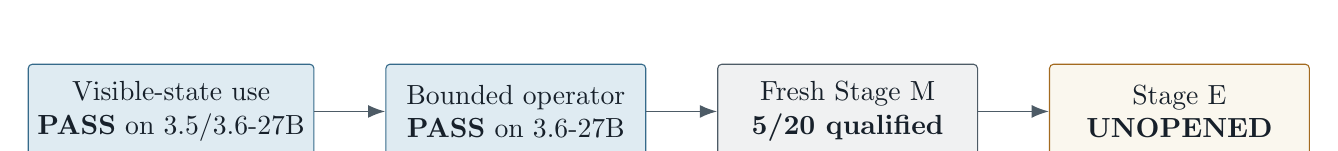
\begin{tikzpicture}[
  node distance=9mm,
  box/.style={draw=Rule, rounded corners=1.5pt, minimum width=33mm, minimum height=12mm, align=center, fill=white, text=Ink},
  good/.style={box, draw=PassBlue, fill=PassPale},
  stop/.style={box, draw=Slate, fill=FailPale},
  hold/.style={box, draw=Warn, fill=UnopenedPale},
  arrow/.style={-{Latex[length=2.2mm]}, semithick, draw=Slate}
]
\node[good] (a2) {Visible-state use\\\textbf{PASS} on 3.5/3.6-27B};
\node[good, right=of a2] (b) {Bounded operator\\\textbf{PASS} on 3.6-27B};
\node[stop, right=of b] (m) {Fresh Stage M\\\textbf{5/20 qualified}};
\node[hold, right=of m] (e) {Stage E\\\textbf{UNOPENED}};
\draw[arrow] (a2)--(b);
\draw[arrow] (b)--(m);
\draw[arrow] (m)--(e);
\end{tikzpicture}}

\vspace{3mm}
\begin{minipage}[t]{0.58\textwidth}
\textbf{B. Frozen block--layer reproducibility matrix}\par\smallskip
\centering
\fontsize{7.4}{8.5}\selectfont
\begin{tabular}{@{}l r c c c c@{}}
\toprule
Block & $d$ & L21 & L43 & L62 & Joint \\
\midrule
B01 & 2 & \PassCell & \FailCell & \FailCell & \FailCell \\
B02 & 2 & \PassCell & \FailCell & \FailCell & \FailCell \\
B03 & 2 & \FailCell & \PassCell & \FailCell & \FailCell \\
B04 & 2 & \PassCell & \PassCell & \FailCell & \FailCell \\
B05 & 2 & \PassCell & \FailCell & \FailCell & \FailCell \\
\addlinespace[1.5pt]
B06 & 4 & \PassCell & \PassCell & \PassCell & \PassCell \\
B07 & 4 & \FailCell & \PassCell & \FailCell & \FailCell \\
B08 & 4 & \FailCell & \PassCell & \FailCell & \FailCell \\
B09 & 4 & \PassCell & \PassCell & \PassCell & \PassCell \\
B10 & 4 & \FailCell & \PassCell & \PassCell & \FailCell \\
\addlinespace[1.5pt]
B11 & 6 & \FailCell & \PassCell & \FailCell & \FailCell \\
B12 & 6 & \FailCell & \FailCell & \PassCell & \FailCell \\
B13 & 6 & \PassCell & \PassCell & \PassCell & \PassCell \\
B14 & 6 & \PassCell & \PassCell & \PassCell & \PassCell \\
B15 & 6 & \PassCell & \FailCell & \FailCell & \FailCell \\
\addlinespace[1.5pt]
B16 & 8 & \PassCell & \PassCell & \FailCell & \FailCell \\
B17 & 8 & \FailCell & \PassCell & \PassCell & \FailCell \\
B18 & 8 & \FailCell & \PassCell & \PassCell & \FailCell \\
B19 & 8 & \PassCell & \PassCell & \PassCell & \PassCell \\
B20 & 8 & \FailCell & \PassCell & \FailCell & \FailCell \\
\midrule
Pass count & & 11/20 & 15/20 & 9/20 & \textbf{5/20} \\
\bottomrule
\end{tabular}

\vspace{1mm}
{\scriptsize\textcolor{PassBlue}{$\checkmark$} pass; \textcolor{Slate}{$\times$} fail. Rows remain in frozen depth-major order.}
\end{minipage}\hfill
\begin{minipage}[t]{0.39\textwidth}
\textbf{C. Sensitivity versus re-estimation}\par\smallskip
\centering
\resizebox{0.98\linewidth}{!}{%
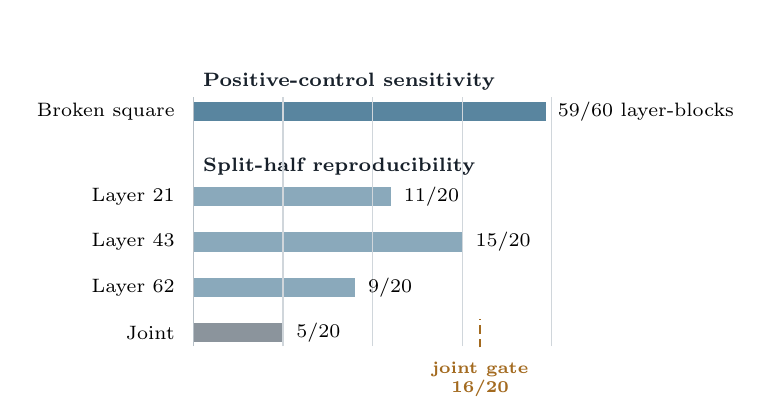
\begin{tikzpicture}[x=4.55cm,y=0.72cm]
  \def\barh{0.34}
  \node[anchor=west,font=\scriptsize\bfseries,text=Ink] at (0,5.35) {Positive-control sensitivity};
  \draw[fill=PassBlue!82,draw=none] (0,4.65) rectangle (0.983,4.65+\barh);
  \node[anchor=east,font=\scriptsize] at (-0.025,4.82) {Broken square};
  \node[anchor=west,font=\scriptsize] at (0.99,4.82) {59/60 layer-blocks};

  \node[anchor=west,font=\scriptsize\bfseries,text=Ink] at (0,3.85) {Split-half reproducibility};
  \draw[fill=PassBlue!58,draw=none] (0,3.15) rectangle (0.55,3.15+\barh);
  \draw[fill=PassBlue!58,draw=none] (0,2.35) rectangle (0.75,2.35+\barh);
  \draw[fill=PassBlue!58,draw=none] (0,1.55) rectangle (0.45,1.55+\barh);
  \draw[fill=Slate!65,draw=none] (0,0.75) rectangle (0.25,0.75+\barh);
  \draw[Rule] (0,0.68) -- (0,5.08);
  \foreach \x in {0.25,0.5,0.75,1.0}{\draw[Rule!65] (\x,0.68)--(\x,5.08);}
  \node[anchor=east,font=\scriptsize] at (-0.025,3.32) {Layer 21};
  \node[anchor=east,font=\scriptsize] at (-0.025,2.52) {Layer 43};
  \node[anchor=east,font=\scriptsize] at (-0.025,1.72) {Layer 62};
  \node[anchor=east,font=\scriptsize] at (-0.025,0.92) {Joint};
  \node[anchor=west,font=\scriptsize] at (0.56,3.32) {11/20};
  \node[anchor=west,font=\scriptsize] at (0.76,2.52) {15/20};
  \node[anchor=west,font=\scriptsize] at (0.46,1.72) {9/20};
  \node[anchor=west,font=\scriptsize] at (0.26,0.92) {5/20};
  \draw[Warn,densely dashed,thick] (0.8,0.66)--(0.8,1.16);
  \node[anchor=north,font=\fontsize{6.2}{6.8}\selectfont\bfseries,text=Warn,align=center] at (0.8,0.58) {joint gate\\16/20};
\end{tikzpicture}}

\vspace{3mm}
\textbf{D. Outcome stage}\par\smallskip
\fcolorbox{Warn}{UnopenedPale}{%
\parbox{0.88\linewidth}{\centering\small
\textbf{Stage E was not opened.}\\[2pt]
Behavior forwards: \textbf{0}\\
$Y_b$: not collected\\
LOBO/permutation test: not run\\
Coupled hypothesis: \textbf{untested}}}
\end{minipage}

\caption{\label{fig:main}\textbf{Sensitivity without reproducibility.} (A) The staged design qualified visible-state use and a bounded operator instrument before opening a prospectively frozen 20-block map requalification. (B) Exact block--layer split-half outcomes; public labels B01--B20 preserve the frozen depth-major order, with exact artifact identifiers reported in Appendix~\ref{app:trackc}. A joint pass required all three frozen layers and no post-hoc block or layer selection. (C) Positive-control sensitivity and split-half re-estimation are visually separated because their denominators differ: 59/60 is a layer-block control count, while 5/20 is the block-level conjunction used for Stage M admission. The dashed marker shows the required joint total; an additional four-per-depth rule also failed. (D) Because the map did not qualify, Stage E remained unopened and the representation--function hypothesis was not tested.}
\end{figure}


\section{Exact Register Square and Staged Claims}
\label{sec:square}

\subsection{Phase-indexed register algebra}

Let the running register be $r_t\in\mathbb F_2$, with visible state
\begin{equation}
  s_t=(t,r_t).
\end{equation}
For an input bit $x\in\mathbb F_2$, define the transition
\begin{equation}
  \tau_{t,x}(t,r)=(t+1,r\oplus x),
\end{equation}
and define a visible counterfactual overwrite
\begin{equation}
  J_t(t,r)=(t,r\oplus 1).
\end{equation}
The phase coordinate prevents the four nodes from collapsing into a two-state diagram. At the external task level, the two paths commute exactly:
\begin{equation}
  \boxed{J_{t+1}\circ\tau_{t,x}=\tau_{t,x}\circ J_t.}
  \label{eq:naturality}
\end{equation}
Writing
\begin{align}
  A&=(t,r), & B&=(t,r\oplus1),\\
  C&=(t+1,r\oplus x), & D&=(t+1,r\oplus x\oplus1),
\end{align}
the paths $A\xrightarrow{J_t}B\xrightarrow{\tau}D$ and $A\xrightarrow{\tau}C\xrightarrow{J_{t+1}}D$ have the same source and target. Equation~\eqref{eq:naturality} is an exact property of the task generator. It does not assert that any internal neural coordinate system realizes an exact commuting square.

\subsection{Conditional evidential ladder}

The study separates five claims. A0 asks whether the checkpoint follows an explicitly available transition rule in one-step and self-fed rollouts. A1 removes the explicit rule and asks whether correct opaque-codebook demonstrations support the frozen register behavior beyond matched controls. A2 applies an explicit overwrite to the visible register and asks whether the immediate successor, downstream states, and final answer change as the external algebra requires while a marker-only control leaves them unchanged. B asks whether a local-frame paired ridge operator packet is independently re-estimable and distinguishes a matched broken-square control on a bounded substrate. C would ask whether a frozen representation-return feature predicts a frozen functional discrepancy over independent fresh blocks.

The order is substantive. A0 failure prevents interpretation of A1 or A2. A1 failure prevents A2. A2 qualifies visible written-state use but does not identify a hidden causal variable. B is observational representation geometry; it is not opened as a causal-transition analysis merely because A2 passes. Finally, the functional C analysis is conditional on fresh map qualification. The paper's terminal result is that the map failed this final prerequisite.

\begin{figure}[ht]
\centering
\begin{minipage}[t]{0.48\textwidth}
\textbf{A. Exact external register square}\par\smallskip
\centering
\resizebox{0.94\linewidth}{!}{%
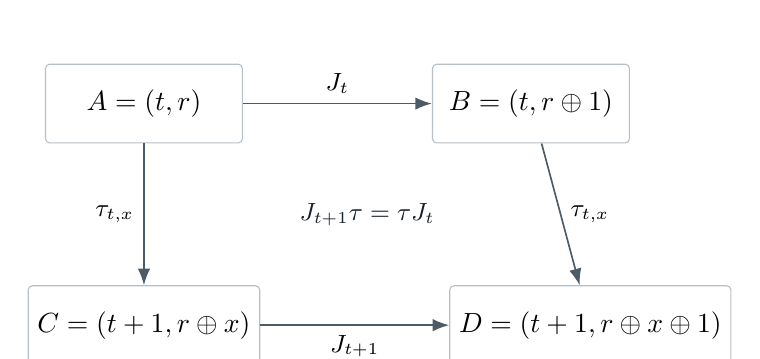
\begin{tikzpicture}[
  node distance=18mm and 24mm,
  state/.style={draw=Rule,rounded corners=1.5pt,minimum width=25mm,minimum height=10mm,fill=white,align=center},
  arr/.style={-{Latex[length=2.1mm]},semithick,draw=Slate}
]
\node[state] (A) {$A=(t,r)$};
\node[state,right=of A] (B) {$B=(t,r\oplus1)$};
\node[state,below=of A] (C) {$C=(t+1,r\oplus x)$};
\node[state,right=of C] (D) {$D=(t+1,r\oplus x\oplus1)$};
\draw[arr] (A)--node[above,font=\small]{$J_t$}(B);
\draw[arr] (A)--node[left,font=\small]{$\tau_{t,x}$}(C);
\draw[arr] (B)--node[right,font=\small]{$\tau_{t,x}$}(D);
\draw[arr] (C)--node[below,font=\small]{$J_{t+1}$}(D);
\node[font=\small,text=Ink,align=center] at ($(A)!0.5!(D)$) {$J_{t+1}\tau=\tau J_t$};
\end{tikzpicture}}
\end{minipage}\hfill
\begin{minipage}[t]{0.49\textwidth}
\textbf{B. Evidential ladder and terminal boundary}\par\smallskip
\centering
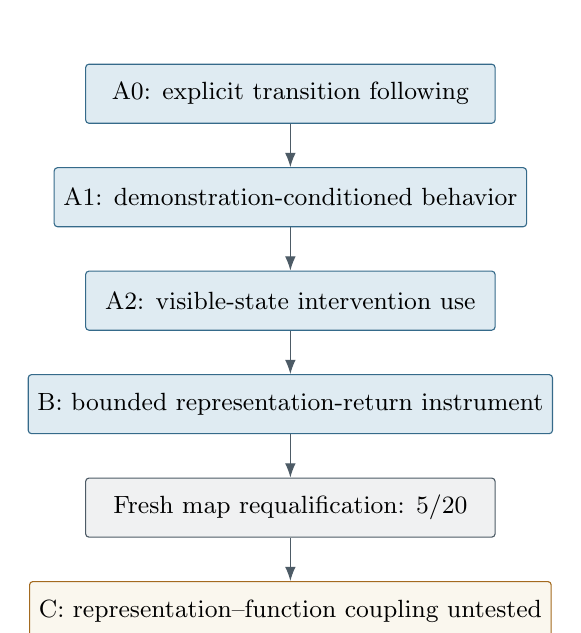
\begin{tikzpicture}[
  node distance=5.5mm,
  stagebox/.style={draw=Rule,rounded corners=1.2pt,minimum width=52mm,minimum height=7.5mm,fill=white,align=center,font=\small},
  good/.style={stagebox,draw=PassBlue,fill=PassPale},
  stop/.style={stagebox,draw=Slate,fill=FailPale},
  hold/.style={stagebox,draw=Warn,fill=UnopenedPale},
  arr/.style={-{Latex[length=1.8mm]},draw=Slate}
]
\node[good] (a0) {A0: explicit transition following};
\node[good,below=of a0] (a1) {A1: demonstration-conditioned behavior};
\node[good,below=of a1] (a2) {A2: visible-state intervention use};
\node[good,below=of a2] (b) {B: bounded representation-return instrument};
\node[stop,below=of b] (m) {Fresh map requalification: 5/20};
\node[hold,below=of m] (c) {C: representation--function coupling untested};
\draw[arr] (a0)--(a1); \draw[arr] (a1)--(a2); \draw[arr] (a2)--(b); \draw[arr] (b)--(m); \draw[arr] (m)--(c);
\end{tikzpicture}
\end{minipage}
\caption{\label{fig:square}\textbf{Exact task algebra and conditional claim ladder.} The external paths commute exactly, but this does not imply exact commutation of an internal representation. The ladder separates intervention-backed visible-state use from observational representation geometry. The terminal boundary occurred at fresh map requalification, before any representation--function coupling analysis.}
\end{figure}


\subsection{Claim boundary}

Only the visible written-state edit is intervention-backed. The operator packet is computed from activation clouds and coordinate relations; it is not a low-level intervention map. Consequently, even a positive B or C result would be weaker than causal abstraction as tested by interchange interventions~\cite{geiger2021,geiger2023das}. In the present study C was not reached, so the strongest supported causal language remains \emph{visible-state intervention use}.

\section{Visible-State Use Qualified at Two Checkpoints}
\label{sec:behavior}

\subsection{Frozen checkpoint panel}

The panel combined a preserved Qwen3-8B baseline with four fresh checkpoints: Qwen3-14B, Qwen3.5-27B, Qwen3.6-27B, and Qwen3.8-27B. Qwen3 introduced supported thinking and non-thinking interaction modes~\cite{yang2025qwen3}; the present study used the frozen non-thinking, forced-choice surface and did not generate a scratchpad. Exact revisions and runtime bindings are reported in Appendix~\ref{app:runtime}. Qwen3.5-27B, Qwen3.6-27B, and Qwen3.8-27B were treated as distinct released checkpoints documented by their official model repositories~\cite{qwen35card,qwen36card,qwen38card}. Their names do not define a controlled training trajectory.

\begin{table}[ht]
\centering
\small
\caption{Frozen behavioral qualification states. \UNOPENED\ means that the downstream surface was not run. The preserved 8B result is historical to the panel but was bound before the fresh checkpoint executions.}
\label{tab:checkpoint-matrix}
\begin{tabular}{@{}lccc@{}}
\toprule
Checkpoint & A0: explicit transition & A1: demonstration-conditioned & A2: visible overwrite \\
\midrule
Qwen3-8B preserved baseline & \PASS & \FAIL & \UNOPENED \\
Qwen3-14B & \FAIL & \UNOPENED & \UNOPENED \\
Qwen3.5-27B & \PASS & \PASS & \PASS \\
Qwen3.6-27B & \PASS & \PASS & \PASS \\
Qwen3.8-27B & \FAIL & \UNOPENED & \UNOPENED \\
\bottomrule
\end{tabular}
\end{table}

\subsection{A0: explicit transition following}

Qwen3.5-27B and Qwen3.6-27B each achieved 32/32 one-step responses, 8/8 in the minimum transition stratum, and 8/8 exact self-fed rollouts. Qwen3-14B achieved 29/32 overall but only 5/8 in the minimum stratum and 5/8 exact rollouts; Qwen3.8-27B achieved 30/32 overall but 6/8 in both corresponding gates. Both therefore failed A0 under the frozen conjunction and were not opened further. Aggregate accuracy could not rescue a failed transition stratum or rollout gate.

\subsection{A1: demonstration-conditioned register behavior}

For Qwen3.5-27B and Qwen3.6-27B, the correct-demonstration condition achieved 16/16 with a 4/4 minimum stratum and exceeded the strongest matched control by 0.50. Corrupted-transition and label-shuffled demonstrations each scored 0/16, while the format-matched control scored 8/16. This is evidence for \emph{demonstration-conditioned register behavior} on the frozen surface, not identification of a unique in-context algorithm or internal implementation.

\subsection{A2: visible overwrite propagation}

The A2 intervention overwrote the visible current register while preserving the next action and protocol. Each call received the current register, the next action, and the frozen context, but no preceding action history. In self-fed continuation, the previous forced-choice state became the next register; after an overwrite, the edited value was therefore the only task-relevant carrier of prior state. In both Qwen3.5-27B and Qwen3.6-27B, the immediate successor was correct in 8/8 cases, all 32/32 downstream states followed the externally implied continuation, and the final state flipped in 8/8 cases; a marker-only control preserved the matched unedited continuation in 40/40 cases. This supports selective use of the written register under the frozen intervention family---the distinction emphasized by controlled-edit work~\cite{somov2026}---but not a hidden register, unique mediation, or an internal realization of Equation~\eqref{eq:naturality}.

\section{A Paired-Map Operator Instrument Qualified on One Bounded Substrate}
\label{sec:operator}

\subsection{Frozen selection and observation surface}

The frozen operator priority was Qwen3.8-27B, Qwen3.6-27B, Qwen3.5-27B, then Qwen3-14B, evaluated only after the checkpoint panel had closed. Qwen3.8-27B failed A0, making Qwen3.6-27B the highest-priority A2-passing checkpoint. The bounded operator study used tuple indices 21, 43, and 62; 24 activation samples per node per independently generated, disjoint half; four nodes from the exact square plus one matched broken-control node; centered rank-4 frames; node-wise orthogonal Procrustes alignment; and frozen paired ridge coordinate maps. Activations were collected at the last prompt position immediately before the forced-choice answer token. The run used 240 unique scientific forwards.

Extraction requested \code{output_hidden_states=True} and indexed the Transformers \code{hidden_states} tuple directly. Under the frozen Transformers 5.15.1 output-capture convention, tuple index 0 is the embedding output and tuple index $k>0$ is the post-block residual output after zero-based decoder block $k-1$; indices 21, 43, and 62 therefore denote the outputs after blocks 20, 42, and 61, before the final model norm. For each tensor the extracted row was \code{hidden_states[k][0,-1,:]}. The BF16 model tensor was cast to PyTorch float32, saved as NumPy float32, and converted to NumPy float64 before centering, ridge fitting, singular-value decomposition, and operator analysis.

Neither rank nor layer was selected from an operator outcome. Rank four was inherited unchanged from the pre-outcome operator-development lock; no empirical rank sweep was used for the bounded run or Stage M. The three layer positions were inherited as normalized depths $1/3$, $2/3$, and $35/36$, then converted by deterministic half-up rounding and clamping to the interior of the checkpoint. For a 64-layer checkpoint this rule yields $[21,43,62]$. All three positions were reported, and no best layer was selected after observation.

For each node $X$, let $U_X\in\mathbb R^{d\times4}$ denote its estimated local frame. Given prospectively paired centered coordinates $X_c,Y_c\in\mathbb R^{n\times4}$ in the source and target frames, respectively, the edge relation was the ridge map
\begin{equation}
 C_{Y\leftarrow X}=Y_c^{\mathsf T}X_c
 \left(X_c^{\mathsf T}X_c+\lambda_X I_4\right)^{-1}.
 \label{eq:ridge-edge}
\end{equation}
Each coordinate-row pair came from the same frozen sample identity: source and target prompts shared the opaque codebook, demonstration identity, action, episode seed, and nuisance half, and differed only in the declared node condition. Thus $C_{Y\leftarrow X}$ maps a source coordinate column toward its paired target coordinate; it is not the raw overlap $U_Y^{\mathsf T}U_X$. The exact regularizer and qualification conventions appear in Appendix~\ref{app:operator}. For the exact square, the two path maps were
\begin{equation}
 P_p=C_{D\leftarrow B}C_{B\leftarrow A},\qquad
 P_q=C_{D\leftarrow C}C_{C\leftarrow A},
 \label{eq:pathmaps}
\end{equation}
\begin{equation}
 \Delta_{p,q}=P_p-P_q.
 \label{eq:delta}
\end{equation}
Under independent orthogonal changes of the source and target frames, $\Delta_{p,q}$ transforms covariantly; its singular values and Frobenius norm are invariant derived views. The saved packet retained the path maps, singular spectra, positive-semidefinite polar factors, and qualified whole-path and edge-wise orthogonal returns. No single scalar was treated as the operator itself.

\subsection{Bounded qualification}

The instrument compared exact-square responses with a matched broken square and an independent split-half floor. For rank $r=4$, a response was $\|\Delta\|_F/\sqrt r$. The split-half floor compared the singular spectra of both exact path maps. A layer qualified only if all frames, edges, and path packets qualified, the floor did not exceed 0.20, and both broken-square responses exceeded a threshold determined by the floor, the exact-square responses, and a fixed 0.05 margin. The broken control establishes sensitivity to the prospectively defined semantic break in the square construction. It does not isolate noncommutation from every local representation change induced by the corrupted demonstration token. Appendix~\ref{app:operator} gives the complete formulas and broken-control construction. Table~\ref{tab:initial-operator} reports the bounded result. All three layers qualified; the bounded readiness rule required at least two. The later fresh-block rule required all three because its representation feature had already been fixed as an equal-weight three-layer aggregate.

\begin{table}[ht]
\centering
\caption{Initial bounded Qwen3.6-27B paired-map operator qualification. Each response pair reports the two nuisance halves. The split-half floor is a singular-spectrum disagreement, whereas exact and broken responses are normalized path discrepancies; these quantities are not required to be numerically ordered.}
\label{tab:initial-operator}
\begin{tabular}{@{}rrrrr@{}}
\toprule
Layer & Split-half floor & Broken threshold & Exact-square responses & Broken-square responses \\
\midrule
21 & 0.05980 & 0.11959 & 0.06053 / 0.01742 & 0.22015 / 0.58323 \\
43 & 0.10337 & 0.20674 & 0.02583 / 0.01527 & 0.31516 / 0.36598 \\
62 & 0.07135 & 0.14269 & 0.00467 / 0.01164 & 0.58036 / 0.61604 \\
\bottomrule
\end{tabular}
\end{table}

The bounded PASS justified a fresh distribution-level requalification. It did not estimate how often the map would qualify over independent blocks. It also did not establish generic holonomy, a global atlas, or a causal transition. Related work has developed gauge-aware path and loop statistics for representations~\cite{sevetlidis2026,javidnia2026}; the present object is narrower: one paired ridge path-pair packet under a declared rank, layer set, and square.

\section{Sensitivity Survived, but the Map Did Not Requalify}
\label{sec:fresh}

\subsection{Prospective fresh-block design}

The fresh requalification used one independently generated naturality-square block as one analysis unit. Twenty blocks were frozen before execution, with five blocks at each rollout depth 2, 4, 6, and 8. Every block had a fresh opaque codebook, fresh demonstration identities, fresh seeds, two disjoint map halves, and a separately frozen behavior ledger. Templates, case identities, execution order, layers, rank, thresholds, and the no-replacement rule were bound before the first Stage M response.

Each map block contained 24 samples per node per half across five nodes, giving $24\times5\times2=240$ forwards per block and 4,800 forwards in total. A block first had to pass the complete layer rule at all three frozen layers and yield finite cross-fitted return energies. Stage-level eligibility then required at least 16 of 20 blocks overall and at least four of five at every rollout depth. Only after those count gates passed would representation-feature variance, design rank, leverage, and permutation-support checks be evaluated for the planned downstream analysis. Failed blocks could not be replaced, depth 2 could not be dropped, and a favorable layer could not be selected after inspection.

\subsection{Fresh qualification result}

Stage M completed all 4,800 accepted scientific forwards without preemption, duplicate accepted identifiers, retry, or resume. Five of twenty blocks qualified jointly:
\begin{equation}
  \text{depth 2: }0/5,\quad
  \text{depth 4: }2/5,\quad
  \text{depth 6: }2/5,\quad
  \text{depth 8: }1/5.
\end{equation}
The terminal state was \code{MAP_COMPLETE_NOT_QUALIFIED}. Both the total-count requirement and every per-depth requirement failed.

\subsection{Sensitivity and reproducibility were different gates}

The broken-square positive control remained sensitive in 59 of 60 layer-blocks. All 60 layer-blocks passed node support, frame rank, paired-map rank/conditioning, path-packet construction, and finite cross-fit checks. Independent-half reproducibility of the exact path-map spectra was materially weaker: layer 21 passed in 11/20 blocks, layer 43 in 15/20, and layer 62 in 9/20, for 35/60 reproducible layer-blocks. The single sensitivity failure occurred in a layer-block that also failed reproducibility, so the layer-level PASS count was likewise 35/60. Only 5/20 blocks passed all three layers jointly. The complete gate decomposition is reported in Table~\ref{tab:gate-decomposition}.

The 59/60 and 5/20 counts have different denominators and answer different questions. The first is a layer-block control count. The second is the block-level conjunction required by the prespecified three-layer estimand. Layer 43's post-result 15/20 rate cannot authorize a layer-43-only analysis: such a change would redefine the representation feature after observing its qualification pattern. Likewise, increasing samples, changing rank, excluding depth 2, or analyzing only the five passing blocks would convert a prospectively gated measurement study into post-hoc instrument search.

\subsection{Conditional stop before functional analysis}

Stage E was conditional on successful Stage M qualification. Because the map did not qualify, Stage E executed zero forwards. Let $E_b$ denote the frozen set of 24 behavior episodes for block $b$, and let $m^P_{be}$ and $m^Q_{be}$ be the correct-state logit minus the alternative-state logit at the frozen common endpoint probe under paths $P$ and $Q$, respectively. The functional quantity
\begin{equation}
  Y_b=\sqrt{\frac{1}{|E_b|}\sum_{e\in E_b}
  \left(m^P_{be}-m^Q_{be}\right)^2}
  \label{eq:Yb}
\end{equation}
was never collected. The planned leave-one-block-out predictive comparison and directional Freedman--Lane permutation test~\cite{freedmanlane1983} were never run. There is no observed coefficient, predictive increment, $p$-value, null association, or power statement about an observed outcome.

The correct conclusion is therefore a measurement-boundary result. The frozen paired-map route retained positive-control sensitivity, but its gauge-invariant path-map singular-spectrum re-estimation component did not qualify often enough under the frozen split-half and block-level rule. The representation--function coupling hypothesis remains untested, not rejected.

\section{What Failed, and What Did Not}
\label{sec:claims}

\begin{table}[ht]
\centering
\caption{Final claim ledger. ``Untested'' is not a negative result.}
\label{tab:claim-ledger}
\begin{tabularx}{\textwidth}{@{}Yp{48mm}@{}}
\toprule
Statement & Supported status \\
\midrule
Visible written-register use under the frozen A2 intervention & Supported on Qwen3.5-27B and Qwen3.6-27B \\
Demonstration-conditioned register behavior under the A1 surface & Supported on Qwen3.5-27B and Qwen3.6-27B \\
Bounded operator-instrument qualification & Supported on one Qwen3.6-27B substrate \\
Reusable rank-4, three-layer, paired ridge coordinate-map instrument across the frozen 20-block distribution & Not qualified \\
Representation return predicts functional path discrepancy & Untested \\
Representation return does not predict functional path discrepancy & Untested \\
Hidden causal register & Untested \\
Internal exact naturality & Untested \\
Paired coordinate map is a causal transition & Not supported and not claimed \\
Parameter count causes the checkpoint pattern & Not tested \\
Broader representation geometry lacks useful structure & Not established \\
\bottomrule
\end{tabularx}
\end{table}

The conditional stop is part of the evidence, not an operational omission. Had Stage E been run on five selected blocks, the analysis unit, representation feature, and selection mechanism would all have differed from the frozen design. A result obtained that way would not answer the prospectively stated question. Stopping preserved the distinction between failure to qualify a measurement and failure of the downstream scientific relation.

The closeout is also narrower than a mechanistic null. It closes a specific route: rank-4 frames, three equally required layers, the declared paired ridge coordinate-map construction, independent split halves, and the frozen block distribution. It does not close alternative representation objects, estimator families, hidden-state interventions, or task substrates. Any alternative would require independent motivation and fresh qualification rather than a renamed repair of the closed packet.

\section{Relation to Prior Work}
\label{sec:related}

\paragraph{Intermediate-state use and causal abstraction.}
Interventions on explicit intermediate structures can reveal whether a model uses what it writes rather than merely producing a self-consistent trace~\cite{somov2026}. Our visible overwrite similarly provides an externally checkable counterfactual, but it does not identify an internal variable. Causal-abstraction methods instead align high-level variables with neural representations and test intervention correspondence~\cite{geiger2021}; distributed alignment search extends that program to non-axis-aligned subspaces~\cite{geiger2023das}. The present A2 evidence is deliberately weaker: it concerns use of a written register, with hidden intervention unopened.

\paragraph{Representation similarity and functional grounding.}
Representation measures can disagree even about basic similarity claims, motivating tests of their sensitivity to functional changes and specificity to nonfunctional changes~\cite{ding2021}. Our study applies the same general discipline to a path-operator instrument but adds a preceding requirement: the measurement must be re-estimable across independent local presentations before functional grounding is attempted. The result shows why this ordering matters. A positive control can remain detectable while the measurement object fails the reproducibility gate needed for a block-level functional analysis.

\paragraph{Naturality and path geometry.}
Approximate naturality has recently been operationalized as a comparison between two transformation-preserving paths~\cite{kamitani2026}. Gauge-invariant representation holonomy and sheaf- or atlas-inspired approaches likewise study path dependence under local coordinate choices~\cite{sevetlidis2026,javidnia2026}. Javidnia additionally evaluates finite-sample stability through bootstrap and sample-size analyses within a context-atlas construction. Our prospective question is different: after a bounded paired-map packet qualified, did the \emph{same frozen measurement route} requalify across independently generated exact-square blocks strongly enough to open a separately frozen functional analysis? Naturality and path geometry are not claimed as new; the contribution is this fail-closed coupling of instrument requalification to downstream interpretation.

\paragraph{Prior graph-XOR boundary.}
An earlier technical report found that correct input--output demonstrations made a two-input XOR mapping behaviorally available in Qwen3-4B and Qwen3-8B, but the behavior did not meet the frozen length-8 parity criterion~\cite{kawasaki2026mapping}. The present study does not pool those data. It changes the behavioral substrate by making a phase-indexed register explicit, then separately qualifies visible-state use before opening any representation analysis.

No first-use claim is made for naturality squares, representation holonomy, intermediate-state edits, causal abstraction, or functional grounding. Among the closest 2026 works, representation holonomy has appeared as an ICLR 2026 conference paper, while several others remain preprints. Publication status and exact scope should be re-audited at submission time.

\section{Limitations and Robustness}
\label{sec:limitations}

\begin{enumerate}
\item \textbf{Single model family and bounded checkpoints.} The non-monotonic panel is descriptive. Checkpoints differ in architecture, training, and post-training details; parameter count is not a controlled cause.
\item \textbf{Shared behavioral ledger.} Qwen3.5-27B and Qwen3.6-27B reproduced the same qualification pattern on the same frozen case ledger. This is cross-checkpoint reproduction, not an independently sampled task replication or independent-laboratory replication.
\item \textbf{Visible intervention only.} A2 supports use of the written register under one intervention family. It does not establish a hidden causal register or mediation by a particular internal state.
\item \textbf{One task surface.} The frozen \code{natural_rule_v1} surface and its opaque codebooks do not establish task-general state use.
\item \textbf{One operator family.} The fresh failure closes the rank-4, three-layer, paired ridge coordinate-map route under the frozen construction, not all representation objects.
\item \textbf{Positive-control scope and magnitude.} The broken square was matched in surface structure and serialization, not in effect magnitude. Its 59/60 sensitivity establishes response to the frozen semantic corruption, but does not isolate noncommutation from every local representation change induced by the corrupted token or establish calibrated sensitivity near the exact-square measurement scale.
\item \textbf{Engineering qualification thresholds.} PASS and FAIL are protocol qualifications, not population confidence statements. The 0.20 reproducibility ceiling and 0.05 sensitivity margins were pragmatic instrument-admission criteria frozen before Stage M, not estimates from the fresh outcomes. The 16/20 and four-per-depth floors preserved the planned four-level depth design and its minimum within-depth permutation support; they were admission rules for the planned functional analysis, not estimates of a population success rate.
\item \textbf{Bounded initial B substrate.} The first operator PASS motivated requalification but consisted of one limited substrate. It did not estimate a general qualification probability.
\item \textbf{Stage E unopened.} No functional outcome exists. The study cannot support either a positive or negative representation--function association claim.
\item \textbf{No post-hoc salvage.} Layer 43, rank changes, depth exclusion, added samples, failed-block replacement, and alternative summaries were not used to rescue the route.
\item \textbf{Operational provenance.} Pre-forward corrections and an earlier operator-run preemption are disclosed in Appendix~\ref{app:provenance}. Accepted scientific identifiers were unique, and Stage M itself required no retry or resume.
\end{enumerate}

Robustness here is primarily procedural. Exact model revisions, tokenizer/runtime locks, case identities, execution order, map halves, thresholds, and conditional stopping were fixed before their relevant outcomes. The result is not strengthened by pretending that the failed map is a general impossibility; it is strengthened by leaving the downstream hypothesis unopened.

\section{Conclusion}
\label{sec:conclusion}

This study qualified visible written-state use in Qwen3.5-27B and Qwen3.6-27B and an operator-valued representation instrument on one bounded Qwen3.6-27B substrate. Under a prospectively frozen 20-block requalification, the same route remained sensitive to the broken-square control in 59 of 60 layer-blocks, but its path-map singular spectra passed the frozen cross-half re-estimation gate at all three layers jointly in only 5 of 20 blocks. The predeclared map gate therefore stopped the campaign before behavioral outcomes were collected.

The coupled representation--function hypothesis remains untested. This is narrower than a mechanistic null and more informative than an execution failure: positive-control sensitivity on one substrate did not make this rank-4, three-layer, paired-map observable a reusable measurement object across fresh local presentations. The appropriate next step is not a post-hoc repair of the closed route. Any successor must begin from an independently motivated measurement principle and qualify that object on fresh data before using it to support a mechanistic claim.

\section*{Data, Code, and Status}

Scientific code, frozen protocol files, and the terminal closeout are available from the public repository at \url{https://github.com/Udonburo/pale-ale}, with the execution record fixed at commit \hash{407d20fd4f074b9ef4524c82c8136874efaec476}. The Zenodo release accompanying this report contains a model-forward-free reproducibility capsule, exact model and runtime identities, the 20-block and 60 layer-block qualification records, deterministic Figure~\ref{fig:main} and Table~\ref{tab:gate-decomposition} inputs, licenses, and top-level \code{SHA256SUMS}. The continuous Stage M fields are exposed in \code{stage_m_layer_block_records.csv} and a matching JSON record, both derived by a source-hash-locked model-free exporter. Its archival DOI is inserted in the release build after reservation. No additional model execution or activation extraction was performed during manuscript assembly, and no inferential outcome analysis was opened.

\small
\begin{thebibliography}{99}

\bibitem{yang2025qwen3}
A. Yang et al.
\newblock Qwen3 Technical Report.
\newblock \emph{arXiv preprint arXiv:2505.09388}, 2025.
\newblock \url{https://arxiv.org/abs/2505.09388}.

\bibitem{qwen35card}
Qwen Team.
\newblock Qwen3.5-27B model card and repository.
\newblock Hugging Face, 2026. Frozen study revision \code{fc05daec18b0a78c049392ed2e771dde82bdf654}.
\newblock \url{https://huggingface.co/Qwen/Qwen3.5-27B}.

\bibitem{qwen36card}
Qwen Team.
\newblock Qwen3.6-27B model card and repository.
\newblock Hugging Face, 2026. Frozen study revision \code{6a9e13bd6fc8f0983b9b99948120bc37f49c13e9}.
\newblock \url{https://huggingface.co/Qwen/Qwen3.6-27B}.

\bibitem{qwen38card}
Qwen Team.
\newblock Qwen3.8-27B model card and repository.
\newblock Hugging Face, 2026. Frozen study revision \code{1d4bf0f2ff6012fd82039f2fa52739d0dd7c60c0}.
\newblock \url{https://huggingface.co/Qwen/Qwen3.8-27B}.

\bibitem{geiger2021}
A. Geiger, H. Lu, T. Icard, and C. Potts.
\newblock Causal abstractions of neural networks.
\newblock In \emph{Advances in Neural Information Processing Systems}, volume 34, pages 9574--9586, 2021.

\bibitem{geiger2023das}
A. Geiger, Z. Wu, C. Potts, T. Icard, and N. D. Goodman.
\newblock Finding alignments between interpretable causal variables and distributed neural representations.
\newblock In \emph{Proceedings of the Third Conference on Causal Learning and Reasoning}, volume 236 of \emph{Proceedings of Machine Learning Research}, pages 160--187, 2024.
\newblock \url{https://proceedings.mlr.press/v236/geiger24a.html}.

\bibitem{ding2021}
F. Ding, J.-S. Denain, and J. Steinhardt.
\newblock Grounding representation similarity through statistical testing.
\newblock In \emph{Advances in Neural Information Processing Systems}, volume 34, pages 1556--1568, 2021.

\bibitem{kamitani2026}
Y. Kamitani.
\newblock Beyond object-level alignment: Do brains and DNNs preserve the same transformations?
\newblock \emph{arXiv preprint arXiv:2605.06420}, 2026.
\newblock \url{https://arxiv.org/abs/2605.06420}.

\bibitem{sevetlidis2026}
V. Sevetlidis and G. Pavlidis.
\newblock Gauge-invariant representation holonomy.
\newblock In \emph{Proceedings of the Fourteenth International Conference on Learning Representations}, 2026.
\newblock \url{https://openreview.net/forum?id=czJqKToDGq}.

\bibitem{javidnia2026}
H. Javidnia.
\newblock A gauge theory of superposition: Toward a sheaf-theoretic atlas of neural representations.
\newblock \emph{arXiv preprint arXiv:2603.00824v2}, 2026.
\newblock \url{https://arxiv.org/abs/2603.00824v2}.

\bibitem{somov2026}
O. Somov, M. Chaichuk, G. Ershov, K. Vafin, M. Seleznyov, A. Panchenko, and E. Tutubalina.
\newblock Breaking the chain: A causal analysis of LLM faithfulness to intermediate structures.
\newblock \emph{arXiv preprint arXiv:2603.16475v2}, 2026.
\newblock \url{https://arxiv.org/abs/2603.16475v2}.

\bibitem{kawasaki2026mapping}
A. Kawasaki.
\newblock Local Mapping Without Iterative Closure: Zero-Shot and Input-Output-Only In-Context Graph-XOR Capability Boundaries in Qwen3.
\newblock Technical note, Zenodo, 2026.
\newblock \url{https://doi.org/10.5281/zenodo.21992852}.

\bibitem{schonemann1966}
P. H. Sch\"onemann.
\newblock A generalized solution of the orthogonal Procrustes problem.
\newblock \emph{Psychometrika}, 31:1--10, 1966.

\bibitem{freedmanlane1983}
D. Freedman and D. Lane.
\newblock A nonstochastic interpretation of reported significance levels.
\newblock \emph{Journal of Business \& Economic Statistics}, 1(4):292--298, 1983.

\end{thebibliography}

\appendix
\footnotesize

\section{Behavioral Protocol and Runtime Bindings}
\label{app:runtime}

\subsection{Checkpoint identities}

\begin{table}[H]
\centering
\caption{Exact checkpoint revisions. The 8B row is a preserved baseline bound from the preceding campaign rather than a new execution in this panel.}
\label{tab:revisions}
\begin{tabularx}{\textwidth}{@{}lY@{}}
\toprule
Checkpoint & Frozen revision \\
\midrule
Qwen3-8B preserved baseline & \hash{b968826d9c46dd6066d109eabc6255188de91218} \\
Qwen3-14B & \hash{40c069824f4251a91eefaf281ebe4c544efd3e18} \\
Qwen3.5-27B & \hash{fc05daec18b0a78c049392ed2e771dde82bdf654} \\
Qwen3.6-27B & \hash{6a9e13bd6fc8f0983b9b99948120bc37f49c13e9} \\
Qwen3.8-27B & \hash{1d4bf0f2ff6012fd82039f2fa52739d0dd7c60c0} \\
\bottomrule
\end{tabularx}
\end{table}

Models were loaded unquantized in BF16 with frozen weights. The preserved Qwen3-8B baseline used an NVIDIA L40S (driver 580.95.05) with Python 3.11.2, PyTorch 2.7.1+cu126, CUDA 12.6, Transformers 5.15.0, tokenizers 0.22.2, SDPA attention, and TF32 disabled. Qwen3-14B used an NVIDIA L40S with the same software versions. The 27B panel and operator runs used an NVIDIA A100-80GB with the same Python, PyTorch, CUDA, and tokenizers versions and Transformers 5.15.1 at commit \hash{550d7b3834670483a4df436541272c055dc364bf}. The forced-choice score used the first semantic assistant-answer token at the validated score slot. Generation, sampling, generated chain-of-thought, and quantization were absent.

The 27B checkpoints are documented as multimodal image--text-to-text models~\cite{qwen35card,qwen36card,qwen38card}, but this study used their frozen text-only path exclusively. No image, video, dummy visual input, or visual placeholder token was supplied.

\subsection{A0--A2 case structure}

A0 used 80 calls per fresh checkpoint: 32 independent teacher-forced one-step calls plus eight exact self-fed rollouts, four of length 4 and four of length 8, totaling $32+4\times4+4\times8=80$ calls. A1 used 64 calls: 16 correct demonstrations and three named 16-case controls (corrupted transition, label-shuffled, and format-matched). A2 used 88 calls organized as eight paired trajectories; each pair contained one shared pre-edit step, five edited continuation steps, and five marker-only continuation steps. Its metric denominators were eight immediate successors, 32 later downstream steps, eight final-state flips, and 40 marker-only no-change steps. Thus a checkpoint reaching A2 used at most 232 new behavioral calls. No failed upstream checkpoint was opened downstream.

\begin{table}[H]
\centering
\scriptsize
\caption{Frozen behavioral qualification rules. Every condition in a row was conjunctive; aggregate accuracy could not rescue a failed stratum, rollout, control, or intervention component.}
\label{tab:behavioral-thresholds}
\begin{tabularx}{\textwidth}{@{}lY@{}}
\toprule
Stage & PASS conditions \\
\midrule
A0 & one-step accuracy $\geq0.90$; minimum frozen transition-cell accuracy $\geq0.80$; exact self-fed rollout accuracy $\geq0.75$ \\
A1 & correct-demonstration accuracy $\geq0.85$; correct minus strongest-control accuracy $\geq0.20$; minimum correct transition-cell accuracy $\geq0.75$; every control accuracy strictly below $0.85$ \\
A2 & edited immediate-successor accuracy $\geq0.90$; edited downstream-step accuracy $\geq0.75$; paired final-state flip rate $\geq0.80$; marker-only no-change accuracy $\geq0.90$ \\
\bottomrule
\end{tabularx}
\end{table}

Every A0/A2 transition prompt excluded the preceding input and state history. It contained the frozen demonstration and protocol context, the current visible register, and the next input action; in a self-fed rollout, the previous forced-choice prediction supplied the next current register. The A2 overwrite replaced that carrier under an explicit intervention marker, while the marker-only control preserved its value. This information bottleneck prevents recovery of the pre-edit register by replaying an action history supplied in the same prompt.

The opaque state/action codebook and answer tokens were verified as single tokens at the exact score position for every checkpoint. In A1, the corrupted-transition control replaced every demonstrated target by its complementary state label while preserving the template, input/action rows, row order, row count, output balance, and token count. The label-shuffled control applied the fixed zero-based output-position order $[2,0,3,1]$, preserving the same surface-token multiset and counts while breaking row-to-target associations. For the binary XOR truth table these two constructions render the same complementary output sequence, so they are named strata but not independent control families. The format-matched control preserved the template, codebook, input/action rows, row count, output balance, and token count, but assigned a seed-shuffled balanced output sequence, with a deterministic rotation if it reproduced the correct sequence. The Qwen3.5 and Qwen3.6 controls used identical construction and case counts; token identifiers were recorded per tokenizer revision.

The bounded Qwen3-8B development campaign compared compact-table and natural-language-rule instruments in two 31-call runs before the qualification ledger was opened. The initial eligibility rule admitted the compact-table version; the stricter confirmatory-aligned rule admitted the natural-language version, which was frozen. No prompt development or checkpoint-specific adaptation was performed on Qwen3-14B or any 27B checkpoint.

\section{Operator Construction and Qualification}
\label{app:operator}

\subsection{Frames and coordinate maps}

For each node condition $X$ and nuisance half $h$, let $A_X^{(h)}\in\mathbb R^{n\times d}$ be the activation matrix and $\bar A_X^{(h)}$ its row-centered form. A thin singular-value decomposition
\begin{equation}
 \bar A_X^{(h)}=L_X^{(h)}D_X^{(h)}V_X^{(h)\mathsf T}
\end{equation}
defined the ambient rank-4 frame $U_X^{(h)}=[v_{X,1}^{(h)},\ldots,v_{X,4}^{(h)}]$ from the first four right singular vectors and local coordinates $X_c^{(h)}=\bar A_X^{(h)}U_X^{(h)}$. Column signs were fixed deterministically. The second-half frame was aligned to the first-half frame separately at each node using right orthogonal Procrustes~\cite{schonemann1966} before the split-half comparison.

Model activations were BF16 on device, cast to PyTorch float32 before transfer, stored as NumPy float32 arrays, and cast to NumPy float64 on loading. Centering, frame SVD, Procrustes alignment, ridge fitting, path composition, polar decomposition, and reported operator quantities were all computed in float64.

For prospectively paired source and target coordinate rows $X_c,Y_c\in\mathbb R^{n\times r}$, $r=4$, the directed edge map was Equation~\eqref{eq:ridge-edge}, with
\begin{equation}
 \lambda_X=10^{-3}\max\!\left\{
 \frac{\operatorname{tr}(X_c^{\mathsf T}X_c)}{r},\epsilon_{64}
 \right\}.
 \label{eq:ridge-lambda}
\end{equation}
Here $\epsilon_{64}=\operatorname{finfo}(\texttt{float64}).\texttt{eps}\approx2.22\times10^{-16}$.
The row index is itself part of the estimand: row $j$ in $X_c$ and row $j$ in $Y_c$ came from the same prospectively frozen sample identity, codebook, demonstration, action, episode seed, and nuisance half. Only the source-versus-target node condition changed. The orientation is source-to-target: for a source coordinate column $z_X$, $C_{Y\leftarrow X}z_X$ is the fitted target coordinate. This is a paired ridge regression relation, not the frame overlap $U_Y^{\mathsf T}U_X$. An edge qualified only when all four singular values exceeded $10^{-8}$ and its condition number did not exceed $10^6$. A rank-deficient or ill-conditioned relation could not be promoted to a full orthogonal return; the saved packet used explicit qualification states and absent optional fields rather than arbitrary SVD completion.

For qualified full-rank path maps, the whole-path polar decomposition $P_i=O_iS_i$ separated a positive-semidefinite distortion factor $S_i$ from an orthogonal factor $O_i$. The whole-path relative factor was $H^{\mathrm{path}}_{p,q}=O_q^{\mathsf T}O_p$. Separately, qualifying each edge and multiplying edge-wise orthogonal factors yielded $H^{\mathrm{edge}}_{p,q}$. These are distinct because the polar factor of a product is generally not the product of the polar factors. Both remained secondary packet fields; the raw path pair and $\Delta_{p,q}$ were primary representation objects.

\subsection{Split-half floor and broken square}

The two nuisance halves supplied independent frame and operator estimates. For half $h\in\{1,2\}$, let
\begin{equation}
 d_h^{\mathrm{exact}}=\frac{\|\Delta_h^{\mathrm{exact}}\|_F}{\sqrt r},
 \qquad
 d_h^{\mathrm{broken}}=\frac{\|\Delta_h^{\mathrm{broken}}\|_F}{\sqrt r}.
 \label{eq:normalized-responses}
\end{equation}
Writing $\sigma(P)$ for the singular-value vector of a path map, the split-half floor was
\begin{equation}
 f=\max_{i\in\{p,q\}}
 \frac{\|\sigma(P_i^{(1)})-\sigma(P_i^{(2)})\|_2}{\sqrt r},
 \label{eq:split-floor}
\end{equation}
and the broken-square sensitivity threshold was
\begin{equation}
 \theta=\max\!\left\{2f,\ f+0.05,\
 \max_h d_h^{\mathrm{exact}}+0.05\right\}.
 \label{eq:broken-threshold}
\end{equation}
The frozen layer rule was
\begin{align}
 \mathrm{REPRODUCIBLE}&\iff f\leq0.20,\\
 \mathrm{SENSITIVE}&\iff \min_h d_h^{\mathrm{broken}}>\theta,\\
 \mathrm{LAYER\_PASS}&\iff
 \mathrm{PACKETS\_QUALIFIED}\land
 \mathrm{REPRODUCIBLE}\land\mathrm{SENSITIVE}.
 \label{eq:layer-pass}
\end{align}
Here \code{PACKETS_QUALIFIED} required node support, rank-4 frames, qualified paired ridge edges, and qualified exact and broken path packets in both halves. The initial bounded instrument passed when at least two of the three frozen layers passed. The later Stage M block rule was stricter:
\begin{equation}
 \mathrm{BLOCK\_PASS}_b\iff
 \bigwedge_{\ell\in\{21,43,62\}}
 \left(\mathrm{LAYER\_PASS}_{b\ell}
 \ \land\ \mathrm{FINITE\_CROSSFIT}_{b\ell}\right).
 \label{eq:block-pass}
\end{equation}
For a given $(b,\ell)$, \code{FINITE_CROSSFIT} required both training-half return-action energies to be present and finite. Each term used a qualified training-half exact packet and rank-4 orthonormal source frame, projected the opposite-half source activations into that frame, and required a positive held-out covariance trace above the frozen floor $10^{-12}\max\{1,\operatorname{mean}(Z^2)\}$. The numerator $\operatorname{tr}(\Delta\Sigma\Delta^{\mathsf T})$ had to be finite and at least $-10^{-10}$; a negative value within that numerical tolerance was clamped to zero. Thus each block required six finite terms---two halves at each of three layers---with no missing packet.
The change was prospective rather than a response to the bounded result. The initial two-of-three conjunction was an instrument-readiness gate. Before Stage M, the downstream representation amplitude was fixed as an equal-weight aggregate over layers 21, 43, and 62; a missing layer would therefore change the estimand. Each fresh block consequently had to supply a valid measurement at all three layers.

Thus an exact response need not lie below $f$: $f$ measures cross-half singular-spectrum disagreement, while $d_h^{\mathrm{exact}}$ measures within-half path discrepancy and enters $\theta$ explicitly. This distinction explains, for example, the layer-21 bounded PASS despite $0.06053$ being slightly larger than $0.05980$.

\paragraph{Exact broken-control construction.}
Let the four correct demonstration rows be
\begin{equation}
 \mathcal D=\bigl((s_j,a_j,o_j)\bigr)_{j=1}^{4},
 \qquad o_j=s_j\oplus a_j,
\end{equation}
where $s_j,a_j,o_j\in\mathbb F_2$ are the semantic state, action, and next-state bits, each rendered by its assigned opaque label. The broken context was constructed deterministically as
\begin{equation}
 \mathcal D^{\times}=\bigl((s_1,a_1,\bar o_1),(s_2,a_2,o_2),
 (s_3,a_3,o_3),(s_4,a_4,o_4)\bigr),
 \qquad \bar o_1=1-o_1
 \label{eq:broken-context}
\end{equation}
after semantic decoding of the opaque labels. In the renderer this means replacing only the first demonstration's output token by the complementary state-label token. The template, codebook, four-row order, row count, allowed state/action sets, protocol phase, queried current state, next action, answer prefix, score slot, and rendered token count were unchanged. Thus $\mathcal D^{\times}$ no longer presents the exact transition table $\tau$, while retaining the same prompt skeleton and one-token answer interface.

The exact registry used
\begin{align}
 p&=(\texttt{phase0\_state0},\texttt{phase0\_state1},\texttt{phase1\_state1}),\\
 q&=(\texttt{phase0\_state0},\texttt{phase1\_state0},\texttt{phase1\_state1}),
\end{align}
whereas the positive control kept $p$ and replaced only the final node of $q$ by \texttt{phase1\_state1\_broken}, rendered with $\mathcal D^{\times}$. The resulting path pair is intentionally not an exact square under the demonstrated transition context. It served as a strong semantic positive control, not as a serialization control and not as a calibrated near-null perturbation. Exact P/Q behavior renderings were separately validated to match on all frozen surface fields, with operation order as the intended difference.

\paragraph{Origin of the admission thresholds.}
The ceiling $f\leq0.20$, the factor $2f$, and the absolute 0.05 margins were pragmatic engineering criteria inherited from the bounded operator lock and frozen before Stage M. They were not estimated from the 20-block outcomes, and they are neither confidence limits nor population error rates. The multiplier required the broken response to exceed twice the self-estimation floor; the two 0.05 terms required an absolute separation from both the floor and the largest exact-square response. At the campaign level, 16/20 with at least four blocks at each of four depths was the minimum complete downstream design: it allowed at most one loss per depth while retaining categorical depth adjustment and at least $(4!)^4-1=331{,}775$ nonidentity within-depth permutations. Model-free audits of the balanced 16- and 20-block designs were completed before execution; no threshold was changed after Stage M.

\section{Fresh Stage M and the Unopened Stage E}
\label{app:trackc}

\subsection{Block and nuisance-half separation}

Table~\ref{tab:separation-contract} records which factors were matched and which were regenerated. ``Independently generated'' means deterministically disjoint identifiers and seed roots under the frozen compiler; it does not assert population-level or stochastic independence. The two halves deliberately shared the task algebra, renderer, and block codebook so that they estimated the same block-level object.

\begin{table}[H]
\centering
\scriptsize
\caption{Frozen sharing and separation contract. ``Shared'' means byte- or semantics-matched as applicable; ``disjoint'' means distinct frozen identities or seed roots.}
\label{tab:separation-contract}
\begin{tabularx}{\textwidth}{@{}Yp{35mm}p{35mm}p{35mm}@{}}
\toprule
Factor & Within paired node rows & Across map halves & Across blocks \\
\midrule
External square algebra and node registry & shared; node condition is the paired difference & shared & shared task family \\
Renderer/template and score slot & shared & shared & shared \\
Opaque codebook & shared & shared within block & regenerated; distinct block identity \\
Map demonstration identity & shared within paired row & disjoint & disjoint \\
Map sample ID and episode seed & shared within paired row & disjoint seed roots & disjoint \\
Behavior ledger & not used in Stage M & disjoint from both map halves & disjoint; remained unopened \\
\bottomrule
\end{tabularx}
\end{table}

\subsection{Frozen Stage M ledger}

The 20 public block identifiers B01--B20 follow the frozen depth-major source order, five per depth. The release exporter fixes that one-to-one ordering, and Figure~\ref{fig:main} does not sort blocks by outcome. Each block used 240 map forwards, for 4,800 total. Accepted case identifiers were unique. The result artifacts contained all 4,800 activation hashes and complete case-ID coverage.

\begin{table}[H]
\centering
\small
\caption{Gate-by-gate decomposition of Stage M. Later predictor-geometry gates were not evaluated after the block-count gate failed; they are \UNOPENED, not negative results.}
\label{tab:gate-decomposition}
\begin{tabularx}{\textwidth}{@{}Yp{29mm}p{41mm}p{19mm}@{}}
\toprule
Gate & Unit & Observed & State \\
\midrule
Artifact completeness & campaign & 4,800/4,800 accepted IDs & \PASS \\
P/Q surface contract & rendered pairs & 480/480 matched & \PASS \\
Node support and rank-4 frame qualification & layer-blocks & 60/60 & \PASS \\
Paired-edge rank/conditioning and exact/broken packets & layer-blocks & 60/60 & \PASS \\
Finite cross-fitted return energies & layer-blocks & 60/60 & \PASS \\
Broken-square sensitivity & layer-blocks & 59/60 & 1 fail \\
Split-half singular-spectrum reproducibility & layer-blocks & 35/60 & 25 fail \\
Complete layer rule & layer-blocks & 35/60 & 25 fail \\
All-three-layer block conjunction & blocks & 5/20 & 15 fail \\
Total and per-depth admission & campaign & 5/20; depth counts 0, 2, 2, 1 & \FAIL \\
$R_b$ variance, design rank, leverage, permutation support & campaign & not reached & \UNOPENED \\
\bottomrule
\end{tabularx}
\end{table}

The one broken-sensitivity failure occurred among the 25 nonreproducible layer-blocks, so split-half reproducibility was the limiting layer-level gate: every reproducible layer-block passed the complete layer rule. At the block level, the all-three-layer conjunction then reduced eligibility to 5/20.

\newpage
\subsection{Planned representation and functional estimands}

The downstream analysis was designed but never executed. For block $b$, layer $\ell\in\{21,43,62\}$, and training half $h$, let $\Delta_{b\ell h}$ be the training-half return action and let $\Sigma_{b\ell h}$ be the opposite-half source covariance expressed in that same training-half source frame. The single planned representation amplitude was
\begin{equation}
 R_b=\sqrt{\frac{1}{3}\sum_{\ell}\frac{1}{2}\sum_h
 \frac{\operatorname{tr}(\Delta_{b\ell h}\Sigma_{b\ell h}\Delta_{b\ell h}^{\mathsf T})}
 {\operatorname{tr}(\Sigma_{b\ell h})}}.
 \label{eq:Rb}
\end{equation}
Multiplication across unrelated half gauges was forbidden. The single planned functional outcome was the root-mean-square path-margin discrepancy $Y_b$ in Equation~\eqref{eq:Yb} over 24 behavior episodes per block.

For the four exact-square nodes $\mathcal N=\{A,B,C,D\}$, let $c_{bhns}$ be the target-state logit minus the alternative-state logit in block $b$, half $h$, node $n$, and map sample $s$. The frozen map-derived competence nuisance was
\begin{equation}
 C_b^M=\frac{1}{2}\sum_{h=1}^{2}\left[
 \frac{1}{4\times24}\sum_{n\in\mathcal N}\sum_{s=1}^{24}c_{bhns}
 \right].
 \label{eq:map-competence}
\end{equation}
It used exactly 192 already-required Stage M rows per block and no broken-square or behavior rows. The nuisance model contained an intercept, categorical rollout-depth indicators with depth 2 as reference, and $C_b^M$. The full model added $R_b$. The planned primary statistic was
\begin{equation}
 T_{\mathrm{LOBO}}=1-\frac{\mathrm{SSE}^{\mathrm{LOBO}}_{\mathrm{full}}}
 {\mathrm{SSE}^{\mathrm{LOBO}}_{\mathrm{nuisance}}}.
\end{equation}
A positive result would have required $T_{\mathrm{LOBO}}>0$, a positive full-cohort coefficient for $R_b$, and a one-sided depth-stratified Freedman--Lane permutation $p\leq0.05$~\cite{freedmanlane1983}, with 99,999 permutations and fold-local scaling. The permutation implementation passed a model-free null audit before the campaign. None of these quantities was computed on scientific outcomes because Stage E was unopened.

\section{Operational Provenance and Bound Identities}
\label{app:provenance}

The fresh Stage M execution identifier was \code{bf41b049-f04b-442e-b0bd-05c8adbd4944}. Pre-forward corrections to remote packaging, volume hydration, and model-directory identity were detected before any scientific response. Stage M then completed without preemption, retry, resume, or duplicated accepted response. The provider-displayed incremental usage was USD 6.56, versus a runner estimate of USD 6.5063; both were below the absolute campaign ceiling.

The earlier bounded operator execution experienced one provider preemption after 46 records. Exact resume skipped those accepted identifiers and executed the remaining 194; all 240 accepted identifiers were unique. Non-scientific development incidents are retained in the campaign audit log rather than reproduced in this paper.

One historical root manifest for the Qwen3.6-27B behavioral execution retained the pre-operator SHA-256 \hash{93d837b5e51562d6d3876f30bb1330cff54002f8a368245443846e0999197274} for \code{execution_claim.json}. The later operator terminal appended its terminal-stage label to that shared claim, whose retrieved and independently re-downloaded final SHA-256 is \hash{53d6c77b74bc73ca2a7abfc2b88cb6158316095dbbe3497ee712c999187ed804}. The historical manifest remains immutable; the superseding release provenance records both hashes. The divergence changes no response, activation, metric, or scientific state.

\begin{table}[ht]
\centering
\caption{Selected immutable identities for the fresh requalification and closeout. The complete inventory remains in the bound campaign artifacts.}
\label{tab:hashes}
\begin{tabularx}{\textwidth}{@{}lY@{}}
\toprule
Object & Immutable identifier \\
\midrule
Qwen3.6-27B model revision & \hash{6a9e13bd6fc8f0983b9b99948120bc37f49c13e9} \\
Execution source commit & \hash{ea4558f0fcfd8944499407747615ec5bf41c1542} \\
Sealed map result & \hash{8c56c308856d486b77356a42fe54ef0bea8f91e486dc5dd3820c3a60db5be772} \\
Retrieval inventory & \hash{611ef9e5075c2698e93a42d2ab4d9e7ff3c2b719864d931ea1e01b18934513ae} \\
Terminal closeout & \hash{fcee0f04dfe35ea19fc4e5247909b9e56cccdf6fa6a41ad213842e1e5452e27e} \\
\bottomrule
\end{tabularx}
\end{table}

The closeout forbids reopening this route by weakening the 16/20 or per-depth floors, selecting layer 43, excluding depth 2, replacing failed blocks, running Stage E on the five passing blocks, changing rank or thresholds, or adding checkpoints to rescue the result.

\end{document}
